\section{\texttt{ex020.IPR.xlsm} - Расчет производительности скважины}

Стационарная модель притока к скважине (закон Дарси с поправкой Вогеля) - одна из самых простых и распространенных моделей, широко применяемая в индустрии. \unf{} содержит функции позволяющие упростить расчет индикаторной кривой. Такие функции имеют префикс \mintinline{vb.net}{IPR_} от Inflow Performance Relationship.

Файл примера \mintinline{vb.net}{ex020.IPR.xlsm} можно найти в папке \texttt{exercises} репозитория \unf{} (смотри рис. \ref{ris:Ex20_1}).

\begin{figure}[h!]
	\center{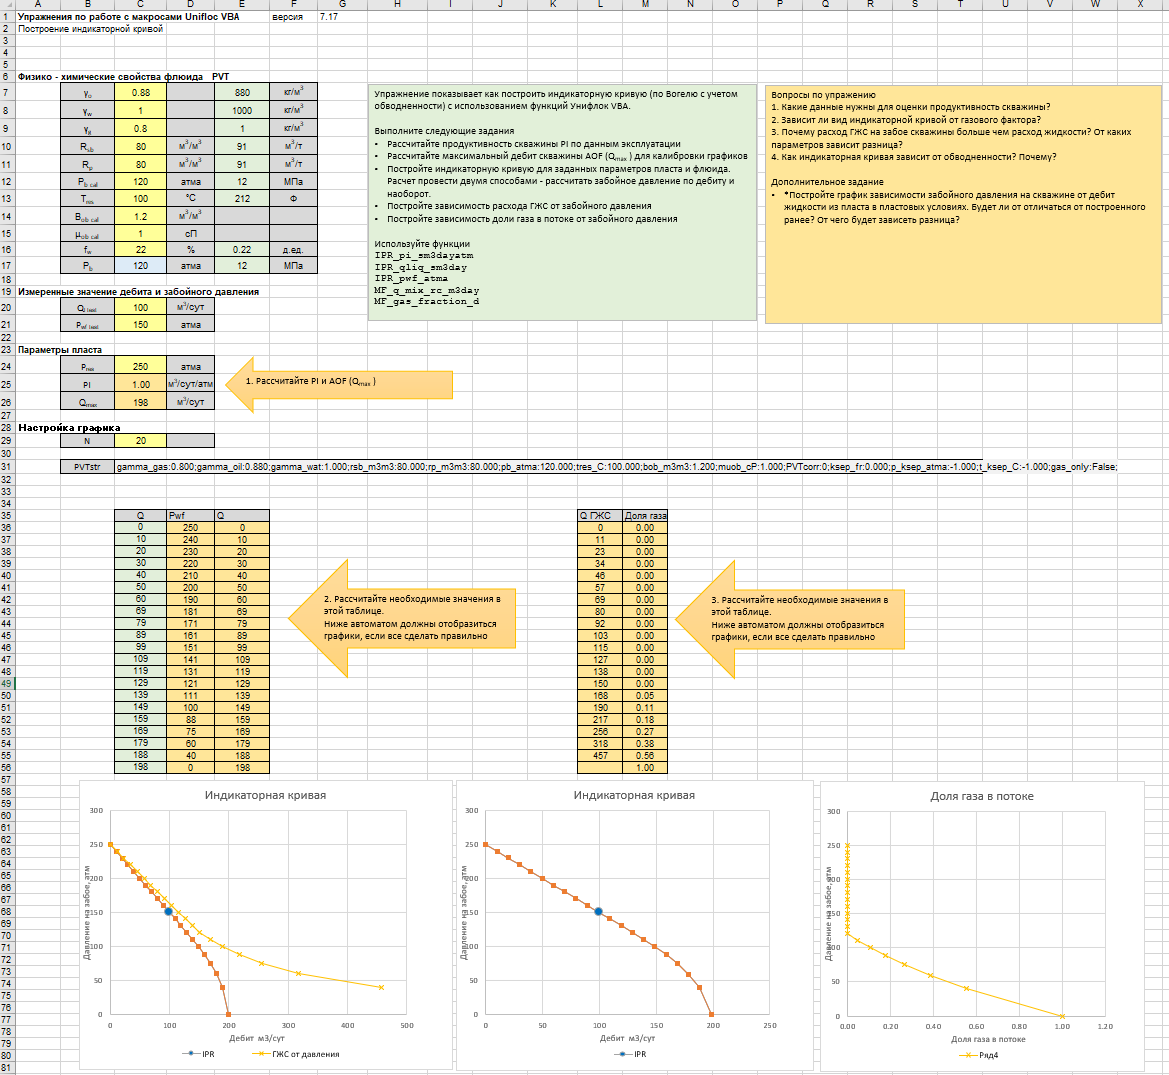
\includegraphics[width=1\linewidth]{Ex20_1}}
	\caption{Упражнение \mintinline{vb.net}{ex020.IPR.xlsx} со всеми заполненными полями }
	\label{ris:Ex20_1}
\end{figure}


\subsection{Упражнение}
Упражнение показывает как построить индикаторную кривую (по Вогелю с учетом обводненности) с использованием функций \unf{}.
 

Выполните следующие задания
\begin{enumerate}
	\item  Рассчитайте продуктивность скважины PI по данным эксплуатации
	\item  Рассчитайте максимальный дебит скважины $AOF=Q_{max}|_{P_{wf}=1}$ для калибровки графиков
	 	 
	\item  Постройте индикаторную кривую для заданных параметров пласта и флюида. Расчет проведите двумя способами - рассчитайте забойное давление по дебиту и наоборот.
	\item  Постройте зависимость расхода ГЖС от забойного давления 
	\item  Постройте зависимость доли газа в потоке от забойного давления
\end{enumerate}


Для выполнения расчетов используйте следующие функции \unf{}:
\begin{itemize}
	
	\item \texttt{IPR\_pi\_sm3dayatm	}
	\item \texttt{IPR\_qliq\_sm3day}
	\item \texttt{IPR\_pwf\_atma}
	\item \texttt{MF\_q\_mix\_rc\_m3day}
	\item \texttt{MF\_gas\_fraction\_d}
	
\end{itemize}


Коэффициент продуктивности $PI$ скважины рассчитывается в ячейке С25 по замеренным данным  с помощью функции

{ \small  \texttt{=IPR\_PI\_sm3dayatm(qltest\_;Pwftest\_;Pres\_;fw\_;Pb\_)}}

А максимальный дебит $Q_{max}$ при максимальной депрессии с забойным давлением равным нулю

{ \small  \texttt{=IPR\_Qliq\_sm3Day(PI\_;Pres\_;0;fw\_;Pb\_)}}


\subsection{Вопросы для самоконтроля}
Для самоконтроля ответьте на следующие вопросы:

\begin{enumerate}
	
	\item Какие данные нужны для оценки продуктивности скважины? Есть два варианта ответа - чем они отличаются между собой?
	
	\item Зависит ли вид индикаторной кривой от газового фактора?
	
	\item Почему расход ГЖС на забое скважины больше чем расход жидкости? От каких параметров зависит разница?
	
  	\item Как индикаторная кривая зависит от обводненности? Почему?
	
	
\end{enumerate}

\subsection{Дополнительные вопросы и задания}

Для того, чтобы глубже разобраться в расчете притока из пласта с использованием \unf{} ответьте на дополнительные вопросы, которые легко превращаются в задания.

\begin{enumerate}
	
	\item  *Постройте график зависимости забойного давления на скважине от дебита жидкости из пласта в пластовых условиях. Будет ли от отличаться от построенного ранее? От чего будет зависеть разница?
	
	
\end{enumerate}